% ==================================================
\section{Эмпирик судалгааны үр дүн}
\label{sec:empirical_results}
% ==================================================

Энэ хэсэгт ковариацын матрицын зургаан үнэлэгчийн
гүйцэтгэлийг корреляцийн бүтэц ялгаатай багцуудад
харьцуулна. Үндсэн шинжилгээнд 120 сарын сургалтын
цонх, 52 сарын түүврээс гадуурх (OOS) өгөөжийг
ашигласан. Үр дүнгийн тогтвортой байдлыг сургалтын
цонхны мэдрэмжийн шинжилгээ, нэмэлт 150 багц болон
bootstrap аргаар шалгав. Мөн тэнцүү жинтэй $1/N$ жишиг багц,
арилжааны зардлын нөлөө болон GMVP--$1/N$
харьцуулалтын bootstrap үр дүнг авч үзэв.


% --------------------------------------------------
\subsection{Ковариацын үнэлэгчдийн OOS гүйцэтгэл}
\label{subsec:oos_performance}
% --------------------------------------------------

Ковариацын үнэлэгчдийн жилд шилжүүлсэн
хэлбэлзэл, харьцангуй дисперсийн бууралт
(RVR) болон Sharpe-ийн харьцааг
Хүснэгт~\ref{tab:oos_performance}-д үзүүлэв.
Энэ хүснэгтэд RVR-ийг Sample үнэлэгчтэй
харьцуулан тооцсон бөгөөд эерэг утга нь
түүврээс гадуурх дисперс буурсныг илэрхийлнэ.

\begin{table}[htbp]
	\centering
	\caption{Ковариацын үнэлэгчдийн OOS гүйцэтгэл ($T=120$)}
	\label{tab:oos_performance}
	\small
	\begin{tabular}{llrrr}
		\hline
		Багц & Үнэлэгч &
		Жилийн хэлбэлзэл & RVR (\%) & Sharpe\\
		\hline
		High & Sample & 0.1705 & 0.00 & 0.7877\\
		& Var  & 0.1655 & 5.81 & 0.8435\\
		& Diag & 0.1678 & 3.18 & 0.8159\\
		& Corr & 0.1716 & -1.26 & 0.8207\\
		& SF   & 0.1666 & 4.56 & 0.8192\\
		& NLS  & 0.1690 & 1.70 & 0.8011\\
		\hline
		Medium & Sample & 0.1428 & 0.00 & 0.6006\\
		& Var  & 0.1427 & 0.15 & 0.6117\\
		& Diag & 0.1426 & 0.35 & 0.6035\\
		& Corr & 0.1412 & 2.26 & 0.5550\\
		& SF   & 0.1416 & 1.65 & 0.5774\\
		& NLS  & 0.1419 & 1.27 & 0.6035\\
		\hline
		Low & Sample & 0.1377 & 0.00 & 0.2687\\
		& Var  & 0.1526 & -22.70 & 0.3925\\
		& Diag & 0.1432 & -8.11 & 0.2549\\
		& Corr & 0.1505 & -19.47 & 0.1109\\
		& SF   & 0.1465 & -13.13 & 0.1905\\
		& NLS  & 0.1399 & -3.24 & 0.3132\\
		\hline
	\end{tabular}
\end{table}

High багцад Var үнэлэгчийн RVR хамгийн
өндөр буюу 5.81\%, Medium багцад Corr
үнэлэгчийнх 2.26\% байна. Харин Low
багцад агшилтын бүх үнэлэгчийн RVR
сөрөг гарч, Sample арга хамгийн бага
OOS дисперстэй байв.

Иймээс анхны гурван багцын хувьд нэг
үнэлэгч бүх нөхцөлд тогтмол давуу
гүйцэтгэл үзүүлээгүй. Эдгээр нь ажиглагдсан
ялгаа бөгөөд статистикийн ач холбогдлыг
дараах шалгалтаар тусад нь үнэлнэ.

% --------------------------------------------------
\subsection{Багцын жингийн тогтвортой байдал}
\label{subsec:portfolio_stability}
% --------------------------------------------------

Багцын жингийн тогтвортой байдлыг дундаж
turnover, төвлөрлийг Херфиндал--Хиршманы
индексээр (HHI) үнэлэв.

\begin{table}[htbp]
	\centering
	\caption{Багцын дундаж turnover болон HHI}
	\label{tab:weight_stability}
	\small
	\begin{tabular}{llrr}
		\hline
		Багц & Үнэлэгч & Turnover & HHI\\
		\hline
		High & Sample & 0.02767 & 0.44468\\
		& Var  & 0.02744 & 0.33715\\
		& Diag & 0.02769 & 0.40338\\
		& Corr & 0.02062 & 0.50315\\
		& SF   & 0.02571 & 0.40821\\
		& NLS  & 0.02757 & 0.40117\\
		\hline
		Medium & Sample & 0.03009 & 0.20008\\
		& Var  & 0.02701 & 0.17750\\
		& Diag & 0.02804 & 0.18949\\
		& Corr & 0.02297 & 0.20775\\
		& SF   & 0.02479 & 0.19316\\
		& NLS  & 0.02603 & 0.18178\\
		\hline
		Low & Sample & 0.02964 & 0.24203\\
		& Var  & 0.02926 & 0.12850\\
		& Diag & 0.02631 & 0.18012\\
		& Corr & 0.02534 & 0.20568\\
		& SF   & 0.02569 & 0.20912\\
		& NLS  & 0.02856 & 0.19904\\
		\hline
	\end{tabular}
\end{table}

Corr үнэлэгч гурван багцад хамгийн бага
turnover, Var үнэлэгч хамгийн бага HHI
үзүүлсэн. Гэвч эдгээр үзүүлэлт бага байх
нь OOS дисперс заавал бага байхыг
илэрхийлэхгүй байна.

% --------------------------------------------------
\subsection{Статистик харьцуулалт}
\label{subsec:statistical_results}
% --------------------------------------------------

Агшилтын үнэлэгчдийн сарын квадрат
өгөөжийн дундаж ялгааг Sample аргатай
HAC шалгалтаар харьцуулж, олон
харьцуулалтад Holm-ийн засвар хэрэглэв.

\begin{table}[htbp]
	\centering
	\caption{Ковариацын үнэлэгчдийн HAC шалгалт ($T=120$)}
	\label{tab:hac_comparison}
	\small
	\begin{tabular}{llrr}
		\hline
		Багц & Үнэлэгч & HAC $p$ & Holm $p$\\
		\hline
		High & Var  & 0.3266 & 0.9799\\
		& Diag & 0.0762 & 0.3048\\
		& Corr & 0.8850 & 0.9799\\
		& SF   & 0.0368 & 0.1842\\
		& NLS  & 0.4639 & 0.9799\\
		\hline
		Medium & Var  & 0.9747 & 1.0000\\
		& Diag & 0.5811 & 1.0000\\
		& Corr & 0.2840 & 1.0000\\
		& SF   & 0.3197 & 1.0000\\
		& NLS  & 0.4438 & 1.0000\\
		\hline
		Low & Var  & 0.0680 & 0.2041\\
		& Diag & 0.0983 & 0.2041\\
		& Corr & 0.0100 & 0.0501\\
		& SF   & 0.0286 & 0.1145\\
		& NLS  & 0.1995 & 0.2041\\
		\hline
	\end{tabular}
\end{table}

Holm-ийн засварын дараа бүх $p$-утга
0.05-аас их байна. Иймээс анхны гурван
багцад квадрат өгөөжийн дундаж ялгаа
5\%-ийн түвшинд статистикийн хувьд
ач холбогдолтой болох нь тогтоогдсонгүй.


% --------------------------------------------------
\subsection{Сургалтын цонхны мэдрэмжийн шинжилгээ}
\label{subsec:sensitivity_results}
% --------------------------------------------------

Сургалтын цонхны уртыг $T=60,90,120$ сар болгон
өөрчилж, ижил 52 сарын түүврээс гадуурх (OOS)
хугацаанд ковариацын үнэлэгчдийн гүйцэтгэлийг
харьцуулав. Хөрөнгийн тоо $N=10$ тогтмол тул
харгалзах $N/T$ харьцаа нь 0.1667, 0.1111,
0.0833 байна. Үр дүнг
Хүснэгт~\ref{tab:nt_sensitivity} болон
Зураг~\ref{fig:nt_rvr_comparison}-т үзүүлэв.

\begin{table}[htbp]
	\centering
	\caption{Сургалтын цонхны уртаас хамаарах RVR (\%)}
	\label{tab:nt_sensitivity}
	\small
	\begin{tabular}{llrrrrr}
		\hline
		Багц & $T$ & Var & Diag & Corr & SF & NLS\\
		\hline
		High & 60  & 3.76 & 2.29 & 6.60 & 3.73 & 5.86\\
		& 90  & 9.21 & 4.90 & -1.65 & 6.28 & 4.54\\
		& 120 & 5.81 & 3.18 & -1.26 & 4.56 & 1.70\\
		\hline
		Medium & 60  & 1.03 & 1.09 & 5.58 & 3.78 & 0.90\\
		& 90  & -0.02 & 0.46 & 3.31 & 1.66 & 0.31\\
		& 120 & 0.15 & 0.35 & 2.26 & 1.65 & 1.27\\
		\hline
		Low & 60  & -27.54 & -10.65 & -18.29 & -17.36 & -10.81\\
		& 90  & -27.12 & -9.23 & -22.68 & -18.64 & -4.55\\
		& 120 & -22.70 & -8.11 & -19.47 & -13.13 & -3.24\\
		\hline
	\end{tabular}
\end{table}

\begin{figure}[htbp]
	\centering
	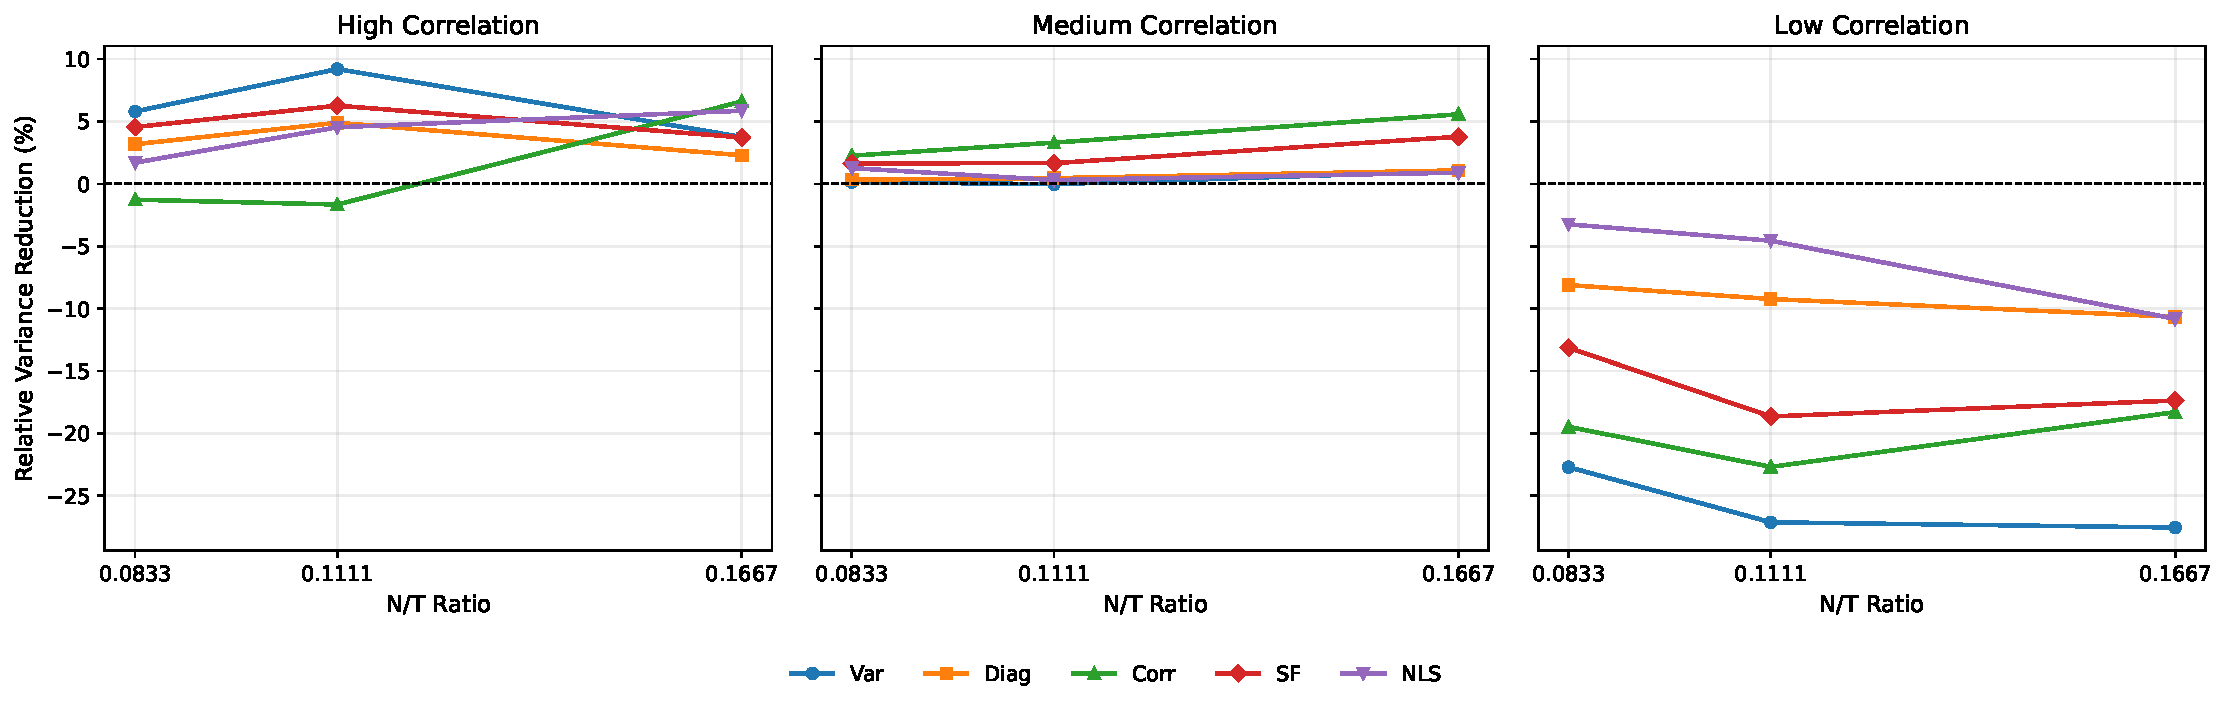
\includegraphics[width=\textwidth]
	{RVR_NT_Three_Portfolios.pdf}
	\caption{Корреляцын бүтэц ялгаатай гурван багцын
		$N/T$ харьцаанаас хамаарах RVR}
	\label{fig:nt_rvr_comparison}
\end{figure}

Зураг~\ref{fig:nt_rvr_comparison}-ээс харахад
High багцад Corr үнэлэгчээс бусад аргууд бүх
сургалтын цонхонд эерэг RVR үзүүлсэн боловч
хамгийн сайн үнэлэгч $N/T$ харьцаанаас
хамааран өөрчлөгдөж байна. Medium багцад
RVR-ийн хэмжээ харьцангуй бага бөгөөд
Corr үнэлэгч бүх цонхонд хамгийн өндөр
дисперсийн бууралт үзүүлэв. Харин Low
багцад бүх агшилтын үнэлэгчийн RVR сөрөг байгаа нь
Sample арга бүх цонхонд хамгийн бага
OOS дисперстэй байсныг харуулна.

Ийнхүү агшилтын үнэлэгчдийн гүйцэтгэл
корреляцийн бүтэц болон сургалтын цонхны
уртаас хамааран ялгаатай байна.
Гэхдээ $T$-г өөрчлөхөд сургалтын өгөгдлийн
хугацаа давхар өөрчлөгдөх тул ажиглагдсан
ялгааг зөвхөн $N/T$ харьцааны нөлөө
гэж тайлбарлах боломжгүй.


\paragraph{Мэдрэмжийн шинжилгээний HAC шалгалт.}

Багц тус бүрийн 15 харьцуулалтад
Holm-ийн засвар хэрэглэв.

\begin{table}[htbp]
	\centering
	\caption{Мэдрэмжийн шинжилгээний HAC шалгалт}
	\label{tab:nt_hac_summary}
	\small
	\begin{tabular}{lrlrr}
		\hline
		Багц & $T$ & Үнэлэгч & HAC $p$ & Holm $p$\\
		\hline
		High   & 90  & Diag & 0.0189 & 0.2839\\
		Medium & 90  & Corr & 0.1860 & 1.0000\\
		Low    & 120 & Corr & 0.0100 & 0.1504\\
		\hline
	\end{tabular}
\end{table}

\noindent
\textit{Тайлбар:} Багц тус бүрийн хамгийн
бага засварлаагүй $p$-утгатай хувилбарыг
үзүүлэв.

Holm-ийн засварыг хэрэглэсний дараа 5\%-ийн ач холбогдлын түвшинд статистикийн ач холбогдолтой ялгаа тогтоогдоогүй нь ажиглагдсан гүйцэтгэлийн зөрүүг агшилтын үнэлэгчдийн түүврийн ковариацын аргаас давуу эсвэл сул байгааг нотлох хангалттай статистик үндэслэл гэж үзэх боломжгүйг харуулж байна.

% --------------------------------------------------
\subsection{150 багцын robustness шинжилгээ}
\label{subsec:robustness_results}
% --------------------------------------------------

Үр дүн багцын бүрэлдэхүүнээс хамаарах
эсэхийг шалгах зорилгоор High, Medium,
Low ангилал тус бүрээс 50, нийт 150
багцад шинжилгээг давтав. Ангиллуудын
сургалтын хугацааны дундаж корреляц
харгалзан 0.5267, 0.3036, 0.1346 байв.

\begin{table}[htbp]
	\centering
	\caption{150 багцын дундаж RVR болон эерэг RVR-ийн хувь}
	\label{tab:robustness_rvr}
	\small
	\begin{tabular}{llrr}
		\hline
		Ангилал & Үнэлэгч &
		Дундаж RVR (\%) & Эерэг RVR (\%)\\
		\hline
		High & Var  & 1.13 & 72\\
		& Diag & 0.81 & 82\\
		& Corr & 0.65 & 60\\
		& SF   & 0.53 & 74\\
		& NLS  & 0.39 & 66\\
		\hline
		Medium & Var  & -1.31 & 48\\
		& Diag & 0.57 & 68\\
		& Corr & 0.55 & 54\\
		& SF   & 0.67 & 64\\
		& NLS  & 0.37 & 56\\
		\hline
		Low & Var  & -35.02 & 28\\
		& Diag & -0.61 & 54\\
		& Corr & 0.16 & 64\\
		& SF   & -1.36 & 42\\
		& NLS  & 0.99 & 74\\
		\hline
	\end{tabular}
\end{table}

High ангилалд бүх агшилтын үнэлэгчийн
дундаж RVR эерэг байна. Medium ангилалд
Var-аас бусад үнэлэгчдийн дундаж RVR
эерэг боловч бууралтын хэмжээ бага байв.

Low ангилалд Var үнэлэгчийн дундаж
RVR -35.02\% байгаа бол NLS үнэлэгчийнх
0.99\% байна. Иймээс анхны Low багцад
бүх агшилтын үнэлэгчийн RVR сөрөг
гарсан үр дүн нэмэлт 50 багцад
бүрэн давтагдсангүй.

% --------------------------------------------------
\subsection{Bootstrap итгэх завсар}
\label{subsec:bootstrap_results}
% --------------------------------------------------

Ангилал тус бүрийн дундаж RVR-ийн
тодорхой бус байдлыг зургаан сарын
блоктой, 3000 давталт бүхий circular
moving-block bootstrap аргаар үнэлэв.

\begin{table}[htbp]
	\centering
	\caption{Дундаж RVR-ийн 95\%-ийн bootstrap итгэх завсар}
	\label{tab:bootstrap_rvr}
	\small
	\begin{tabular}{llrrr}
		\hline
		Ангилал & Үнэлэгч &
		RVR (\%) & Доод & Дээд\\
		\hline
		High & Var  & 1.13 & -1.16 & 3.38\\
		& Diag & 0.81 & -0.09 & 1.83\\
		& Corr & 0.65 & -1.83 & 3.45\\
		& SF   & 0.53 & -0.54 & 1.55\\
		& NLS  & 0.39 & -0.45 & 1.40\\
		\hline
		Medium & Var  & -1.31 & -5.08 & 2.55\\
		& Diag & 0.57 & -0.67 & 1.87\\
		& Corr & 0.55 & -0.96 & 1.85\\
		& SF   & 0.67 & -0.39 & 1.46\\
		& NLS  & 0.37 & -0.66 & 1.45\\
		\hline
		Low & Var  & -35.02 & -65.61 & -14.67\\
		& Diag & -0.61 & -5.21 & 3.58\\
		& Corr & 0.16 & -1.95 & 2.15\\
		& SF   & -1.36 & -5.58 & 1.76\\
		& NLS  & 0.99 & -0.52 & 2.41\\
		\hline
	\end{tabular}
\end{table}

Low ангиллын Var үнэлэгчээс бусад
бүх үнэлэгчийн 95\%-ийн итгэх завсар
тэгийг агуулж байна. Харин Low
ангиллын Var үнэлэгчийн итгэх завсар
$[-65.61,-14.67]$ байгаа нь Sample
аргатай харьцуулахад дундаж OOS
дисперс өссөнийг дэмжиж байна.

Иймээс 150 багцын robustness шинжилгээний үр дүнгээр агшилтын үнэлэгчид Sample аргатай харьцуулахад OOS дисперсийг статистикийн хувьд ач холбогдолтойгоор бууруулдаг гэсэн хангалттай нотолгоо тогтоогдсонгүй. Харин Low ангиллын Var үнэлэгчийн дундаж RVR-ийн итгэх завсар тэгийг агуулаагүй бөгөөд энэ нь тухайн ангилалд дисперс өсөх хандлага ажиглагдсаныг илэрхийлнэ. Гэвч уг итгэх завсарт олон харьцуулалтын засвар хийгдээгүй тул энэ үр дүнг олон үнэлэгч, ангиллыг хамарсан статистик дүгнэлтийн түвшинд баталгаатай гэж үзэх боломжгүй.

% --------------------------------------------------
\subsection{Корреляцийн ангилал хоорондын харьцуулалт}
\label{subsec:tier_comparison_results}
% --------------------------------------------------

Агшилтын үнэлэгчдийн дундаж RVR
корреляцийн ангиллаас хамааран ялгаатай
эсэхийг шалгах зорилгоор High--Medium,
High--Low болон Medium--Low гэсэн гурван
хос харьцуулалт хийв. Ангилал бүрд таван
агшилтын үнэлэгчийг авч үзсэн тул нийт
15 харьцуулалт хийгдсэн.

Ангилал хоорондын дундаж RVR-ийн ялгааг
ижил сарын индексүүдээр гүйцэтгэсэн
circular moving-block bootstrap аргаар
үнэлж, 95\%-ийн итгэх завсрыг тооцсон.
Олон харьцуулалтаас үүдэх алдааг
хянахын тулд нийт 15 харьцуулалтын
$p$-утгад Holm-ийн засвар хэрэглэв.

\begin{table}[htbp]
	\centering
	\caption{Корреляцийн ангилал хоорондын
		дундаж RVR-ийн ялгааны bootstrap шинжилгээ}
	\label{tab:tier_comparison}
	\small
	\begin{tabular}{llrrrr}
		\hline
		Харьцуулалт & Үнэлэгч &
		Ялгаа &
		95\% CI доод &
		95\% CI дээд &
		Holm $p$\\
		\hline
		High--Medium
		& Var  &  2.43 & -0.57 &  5.46 & 1.000\\
		& Diag &  0.24 & -0.60 &  1.10 & 1.000\\
		& Corr &  0.10 & -2.62 &  3.32 & 1.000\\
		& SF   & -0.14 & -1.36 &  1.46 & 1.000\\
		& NLS  &  0.02 & -0.95 &  1.07 & 1.000\\
		\hline
		High--Low
		& Var  & 36.15 & 16.55 & 66.37 & 0.220\\
		& Diag &  1.42 & -2.03 &  5.45 & 1.000\\
		& Corr &  0.49 & -1.57 &  2.51 & 1.000\\
		& SF   &  1.89 & -1.67 &  6.82 & 1.000\\
		& NLS  & -0.60 & -1.71 &  0.81 & 1.000\\
		\hline
		Medium--Low
		& Var  & 33.71 & 15.23 & 63.54 & 0.252\\
		& Diag &  1.18 & -1.79 &  4.61 & 1.000\\
		& Corr &  0.39 & -2.45 &  2.81 & 1.000\\
		& SF   &  2.03 & -0.79 &  5.51 & 1.000\\
		& NLS  & -0.62 & -1.38 &  0.18 & 1.000\\
		\hline
	\end{tabular}
\end{table}

\noindent
\textit{Тайлбар:}
Ялгааг эхний ангиллын дундаж RVR-ээс
хоёр дахь ангиллын дундаж RVR-ийг
хасаж тооцсон. RVR-ийн ялгаа болон
итгэх завсрын хязгааруудыг процентын
пунктээр илэрхийлэв.
95\%-ийн итгэх завсрууд нь олон
харьцуулалтын засвар хийгдээгүй
bootstrap итгэх завсар бөгөөд
сүүлийн баганад 15 харьцуулалтад
Holm-ийн засвар хэрэглэсэн
$p$-утгуудыг харуулав.

Хүснэгт~\ref{tab:tier_comparison}-ээс
харахад High--Medium харьцуулалтад
Var үнэлэгчийн дундаж RVR-ийн ялгаа
2.43 процентын пункт байгаа бол
бусад үнэлэгчдийн ялгаа харьцангуй
бага байна. Гэхдээ таван үнэлэгчийн
бүх итгэх завсар тэгийг агуулж,
Holm-ийн засварласан $p$-утгууд
1.000 гарсан тул эдгээр хоёр
ангиллын хооронд статистикийн
ач холбогдолтой ялгаа тогтоогдсонгүй.

Харин High--Low болон Medium--Low
харьцуулалтад Var үнэлэгчийн
дундаж RVR-ийн ялгаа харгалзан
36.15 болон 33.71 процентын пункт
байна. Эдгээр ялгааны засварлаагүй
95\%-ийн bootstrap итгэх завсар
харгалзан [16.55, 66.37] болон
[15.23, 63.54] байгаа нь
хоёулаа тэгийг агуулаагүй.
Энэ нь засварлаагүй шинжилгээний
түвшинд Var үнэлэгчийн дундаж
RVR Low ангилалд High болон
Medium ангиллаас бага байгааг
илэрхийлж байна.

Гэвч олон харьцуулалтын засвар
хэрэглэсний дараа эдгээр хоёр
харьцуулалтын $p$-утга харгалзан
0.220 болон 0.252 болж,
5\%-ийн ач холбогдлын түвшнээс
давсан байна. Иймээс засварлаагүй
итгэх завсрууд тэгийг агуулаагүй
боловч олон харьцуулалтыг
хамтад нь авч үзэхэд эдгээр
ялгааг статистикийн хувьд
ач холбогдолтой гэж дүгнэх
хангалттай үндэслэлгүй байна.

Бусад дөрвөн үнэлэгчийн хувьд
High--Low болон Medium--Low
харьцуулалтын бүх итгэх завсар
тэгийг агуулж байна. Тухайлбал,
NLS үнэлэгчийн High--Low болон
Medium--Low ялгаа харгалзан
-0.60, -0.62 процентын пункт
байгаа боловч эдгээр ялгаа
статистикийн хувьд ач
холбогдолтой биш байна.

Ерөнхийд нь дүгнэвэл,
корреляцийн ангиллуудын хооронд
агшилтын үнэлэгчдийн дундаж
RVR-ийн ялгаа ажиглагдсан
боловч нийт 15 харьцуулалтад
Holm-ийн засвар хэрэглэсний
дараа 5\%-ийн түвшинд
статистикийн ач холбогдолтой
ялгаа тогтоогдсонгүй.
Иймээс корреляцийн ангиллаас
хамааран агшилтын үнэлэгчдийн
гүйцэтгэл ялгаатай байж болох
шинж тэмдэг ажиглагдсан ч
энэхүү ялгааг статистикийн
хувьд баталгаатай гэж
дүгнэх боломжгүй байна.


% --------------------------------------------------
\subsection{Тэнцүү жинтэй багцтай харьцуулалт}
\label{subsec:equal_weight_results}
% --------------------------------------------------

Ковариацын үнэлэгчид суурилсан GMVP-ийн
практик гүйцэтгэлийг үнэлэхийн тулд
хөрөнгө тус бүрд $1/N$ жин оноож,
сар бүр дахин тэнцвэржүүлдэг жишиг
багцтай харьцуулав. Бүх стратегид
үндсэн шинжилгээтэй ижил 52 сарын
OOS хугацааг ашиглав.

\begin{table}[htbp]
	\centering
	\caption{GMVP болон $1/N$ багцын OOS гүйцэтгэл ($T=120$)}
	\label{tab:equal_weight_comparison}
	\small
	\begin{tabular}{llrrr}
		\hline
		Багц & Стратеги &
		Жилийн хэлбэлзэл (\%) &
		$1/N$-тэй харьцуулсан RVR (\%) &
		Sharpe \\
		\hline
		High & Sample & 17.05 & 35.89 & 0.788 \\
		& Var & 16.55 & 39.61 & 0.843 \\
		& Diag & 16.78 & 37.93 & 0.816 \\
		& Corr & 17.16 & 35.08 & 0.821 \\
		& SF & 16.66 & 38.81 & 0.819 \\
		& NLS & 16.90 & 36.98 & 0.801 \\
		& $1/N$ & 21.29 & 0.00 & 0.840 \\
		\hline
		Medium & Sample & 14.28 & 15.72 & 0.601 \\
		& Var & 14.27 & 15.85 & 0.612 \\
		& Diag & 14.26 & 16.02 & 0.603 \\
		& Corr & 14.12 & 17.63 & 0.555 \\
		& SF & 14.16 & 17.11 & 0.577 \\
		& NLS & 14.19 & 16.79 & 0.603 \\
		& $1/N$ & 15.56 & 0.00 & 0.602 \\
		\hline
		Low & Sample & 13.77 & 26.06 & 0.269 \\
		& Var & 15.26 & 9.28 & 0.393 \\
		& Diag & 14.32 & 20.07 & 0.255 \\
		& Corr & 15.05 & 11.67 & 0.111 \\
		& SF & 14.65 & 16.36 & 0.190 \\
		& NLS & 13.99 & 23.67 & 0.313 \\
		& $1/N$ & 16.02 & 0.00 & 0.573 \\
		\hline
	\end{tabular}
\end{table}

Энэ хүснэгтийн RVR-ийг Sample бус, $1/N$
жишиг багцын дисперстэй харьцуулан тооцсон.
Хүснэгт~\ref{tab:equal_weight_comparison}-ээс
харахад гурван багцын хувьд зургаан GMVP
стратеги бүгд $1/N$ жишиг багцаас
бага OOS хэлбэлзэлтэй байна.
$1/N$ багцын жилийн хэлбэлзэл High,
Medium, Low багцад харгалзан
21.29\%, 15.56\%, 16.02\% байв.
Харин хамгийн бага хэлбэлзэлтэй
GMVP стратегиуд нь High багцад Var
(16.55\%), Medium багцад Corr (14.12\%),
Low багцад Sample (13.77\%) байна.

Гэхдээ хэлбэлзлийн давуу байдал нь
Sharpe-ийн харьцаагаар давуу байна
гэсэн үг биш. Тухайлбал, Low багцад
$1/N$ стратегийн Sharpe 0.573 байхад
GMVP стратегиудын Sharpe 0.111--0.393
хооронд байна. Иймээс GMVP-ийн
эрсдэлийг бууруулах зорилгыг
өгөөж--эрсдэлийн харьцааны үнэлгээнээс
тусад нь авч үзэх шаардлагатай.

% --------------------------------------------------
\subsection{Арилжааны зардлын нөлөө}
\label{subsec:trading_cost_results}
% --------------------------------------------------

Сар бүрийн дахин тэнцвэржүүлэлтийн
арилжааны зардлыг тооцохдоо нэг талын
арилжаанд 0, 5, 10, 25 суурь нэгж
(basis points, bps)-ийн хувилбаруудыг
ашиглав. Эхний OOS багц бүрдүүлэлтийн
зардлыг тооцоогүй. Доорх хүснэгтэд
нэг талын 10 bps зардлын хувилбарын
үр дүнг үзүүлэв.

\begin{table}[htbp]
	\centering
	\caption{Нэг талын 10 bps арилжааны зардлын дараах OOS гүйцэтгэл}
	\label{tab:trading_cost_results}
	\small
	\begin{tabular}{llrr}
		\hline
		Багц & Стратеги &
		Цэвэр Sharpe &
		Хуримтлагдсан цэвэр өгөөж (\%) \\
		\hline
		High & Sample & 0.784 & 67.46 \\
		& Var & 0.840 & 71.91 \\
		& Diag & 0.812 & 69.65 \\
		& Corr & 0.818 & 72.27 \\
		& SF & 0.816 & 69.53 \\
		& NLS & 0.797 & 68.45 \\
		& $1/N$ & 0.837 & 96.05 \\
		\hline
		Medium & Sample & 0.596 & 38.36 \\
		& Var & 0.607 & 39.31 \\
		& Diag & 0.599 & 38.56 \\
		& Corr & 0.551 & 34.21 \\
		& SF & 0.573 & 36.15 \\
		& NLS & 0.599 & 38.40 \\
		& $1/N$ & 0.599 & 42.07 \\
		\hline
		Low & Sample & 0.264 & 12.35 \\
		& Var & 0.388 & 22.92 \\
		& Diag & 0.251 & 11.77 \\
		& Corr & 0.107 & 2.13 \\
		& SF & 0.186 & 7.48 \\
		& NLS & 0.308 & 15.57 \\
		& $1/N$ & 0.568 & 40.28 \\
		\hline
	\end{tabular}
\end{table}

Арилжааны зардлыг тусгахад стратегиудын
Sharpe-ийн харьцаа зардалгүй
хувилбартай харьцуулахад бага зэрэг
буурч байна. Тухайлбал, High багцад
Var стратегийн Sharpe 0.843-аас
0.840 болж буурсан. Medium багцад
Var стратегийн цэвэр Sharpe 0.607,
Low багцад $1/N$ стратегийнх 0.568 байна.

High багцад $1/N$ стратегийн
хуримтлагдсан цэвэр өгөөж 96.05\%
байхад Var стратегийнх 71.91\% байна.
Иймээс GMVP стратегиудын хэлбэлзэл
бага байгаа нь хуримтлагдсан өгөөж
өндөр байна гэсэн баталгаа биш.
Эдгээр дүгнэлт нь сонгосон зардлын
хувилбар, сарын дахин тэнцвэржүүлэлт
болон 52 сарын OOS хугацаанд хамаарна.

% --------------------------------------------------
\subsection{GMVP ба $1/N$ багцын bootstrap харьцуулалт}
\label{subsec:bootstrap_equal_weight_results}
% --------------------------------------------------

GMVP стратегиудын $1/N$ жишиг багцтай
харьцуулсан дисперсийн бууралтын
тодорхой бус байдлыг 52 сарын OOS
өгөөжид суурилсан, зургаан сарын
блоктой, 3000 давталт бүхий circular
moving-block bootstrap аргаар үнэлэв.
Сар бүрийн индексүүдийг харьцуулж буй
стратегиудад ижил сонгож,
95\%-ийн percentile итгэх завсар
байгуулав. Багц тус бүрийн зургаан
харьцуулалтын bootstrap $p$-утгад
Holm-ийн засвар хэрэглэв.

\begin{table}[htbp]
	\centering
	\caption{GMVP-ийн $1/N$-тэй харьцуулсан RVR ба bootstrap шалгалт}
	\label{tab:bootstrap_equal_weight}
	\small
	\begin{tabular}{llrrrr}
		\hline
		Багц & Стратеги & RVR (\%) &
		95\% CI доод & 95\% CI дээд & Holm $p$ \\
		\hline
		High & Sample & 35.89 & -21.61 & 63.60 & 0.3149 \\
		& Var & 39.61 & -7.09 & 62.44 & 0.2639 \\
		& Diag & 37.93 & -15.32 & 64.14 & 0.3149 \\
		& Corr & 35.08 & -38.50 & 69.33 & 0.3149 \\
		& SF & 38.81 & -15.41 & 64.90 & 0.3149 \\
		& NLS & 36.98 & -16.53 & 62.84 & 0.3149 \\
		\hline
		Medium & Sample & 15.72 & -4.31 & 31.44 & 0.3399 \\
		& Var & 15.85 & -2.62 & 30.02 & 0.3399 \\
		& Diag & 16.02 & -3.31 & 31.15 & 0.3399 \\
		& Corr & 17.63 & -3.95 & 34.33 & 0.3399 \\
		& SF & 17.11 & -4.21 & 33.32 & 0.3399 \\
		& NLS & 16.79 & -3.61 & 31.72 & 0.3399 \\
		\hline
		Low & Sample & 26.06 & -7.84 & 51.16 & 0.5498 \\
		& Var & 9.28 & -16.30 & 29.00 & 0.8144 \\
		& Diag & 20.07 & -9.26 & 42.20 & 0.5498 \\
		& Corr & 11.67 & -20.01 & 35.14 & 0.8144 \\
		& SF & 16.36 & -18.68 & 40.65 & 0.8107 \\
		& NLS & 23.67 & -8.70 & 47.86 & 0.5498 \\
		\hline
	\end{tabular}
\end{table}

Хүснэгт~\ref{tab:bootstrap_equal_weight}-д
бүх GMVP стратегийн RVR эерэг байна.
Хамгийн бага хэлбэлзэлтэй стратегиудын
$1/N$-тэй харьцуулсан RVR нь High
багцад Var 39.61\%, Medium багцад
Corr 17.63\%, Low багцад Sample
26.06\% байна. Гэвч эдгээрийн
95\%-ийн итгэх завсар харгалзан
$[-7.09,62.44]$, $[-3.95,34.33]$,
$[-7.84,51.16]$ тул тэгийг агуулж байна.

Мөн багц тус бүрийн зургаан
харьцуулалтад Holm-ийн засвар
хэрэглэсний дараа 5\%-ийн түвшинд
статистикийн ач холбогдолтой ялгаа
илрээгүй. Bootstrap $p$-утгыг
төвлөрүүлсэн bootstrap тархалтаас,
харин итгэх завсрыг percentile
аргаар байгуулсан тул засварлаагүй
$p$-утга ба итгэх завсрын шийдвэр
зарим тохиолдолд зөрж болохыг
харгалзан үзнэ. Иймээс ажиглагдсан
эерэг RVR-ийг статистикийн хувьд
баталгаатай давуу байдал гэж
тайлбарлахгүй.

% --------------------------------------------------
\subsection{Үр дүнгийн нэгтгэл}
\label{subsec:results_summary}
% --------------------------------------------------

Эмпирик шинжилгээгээр ковариацын
матрицын агшилтын үнэлэгчдийн
гүйцэтгэл багцын бүрэлдэхүүн болон
сургалтын цонхны уртаас хамааран
ялгаатай байгааг ажиглав.

Анхны гурван багцын HAC шалгалт
болон 150 багцын bootstrap шинжилгээ
нь агшилтын үнэлэгчдийн Sample
аргаас тогтвортой давуу байдлыг
статистикийн хувьд батлаагүй.

Харин бага корреляцтай багцуудад
Var үнэлэгчийн дундаж RVR
мэдэгдэхүйц сөрөг гарсан нь
агшилтын арга бүр OOS эрсдэлийг
бууруулах баталгаагүйг харуулж байна.

Ангилал хоорондын харьцуулалтаар
ажиглагдсан ялгаа олон шалгалтын
засварын дараа статистикийн
ач холбогдолтой болох нь
тогтоогдсонгүй.

$1/N$ жишиг багцтай харьцуулахад
зургаан GMVP стратеги гурван багцад
бүгд бага OOS хэлбэлзэлтэй байсан
боловч bootstrap шалгалтын
олон харьцуулалтын засварын дараа
статистикийн ач холбогдолтой давуу
байдал тогтоогдсонгүй. Мөн
арилжааны зардлыг тооцоход
стратегиудын цэвэр гүйцэтгэл
буурч, хэлбэлзлийн давуу байдал
Sharpe болон хуримтлагдсан
өгөөжийн давуу байдалтай
заавал давхцахгүй байв.

Ковариацын үнэлэгчдийн хоорондын OOS хэлбэлзлийн
ялгаа олон тохиолдолд бага байгаа нь long-only
хязгаарлалттай багцад нэмэлт агшилтын үр ашиг
хязгаарлагдаж болохыг харуулсан
\citet{DeNardKostovic2026}-ийн үр дүнтэй
нийцэж байна. Тэдний судалгаанд багцын жингийн
хязгаарлалт нь өөрөө зохицуулах нөлөө үзүүлж,
ковариацын матрицад нэмэлт агшилт хийх хэрэгцээг
бууруулж болохыг авч үзсэн. Гэхдээ уг судалгаанд
өдрийн өгөөж, илүү олон хөрөнгөтэй багцуудыг
шинжилсэн бол энэхүү судалгаанд зөвхөн сарын
өгөөж, бага $N/T$ харьцаатай 10 хөрөнгийн
багцуудыг ашигласан. Иймээс хоёр судалгааны
үр дүнг шууд ижил нөхцөлийн нотолгоо гэж үзэхгүй.
